\subsection{Golf All the Things}
Golf All the Things is a game currently under development. When my internship started a number of levels had already been made and were being tested. The first levels are similar to an ordinary golf game, but gradually more and more wacky elements are incorporated. In one level, instead of shooting the golf ball across the field, the player propels the golf player himself towards the hole. In another level, the player plays as an elephant being kidnapped by some evil-doers. The general mechanic is that the player touches a point on the screen, moves the finger in the desired direction and lifts the finger. The line between the initial point and the point of release defines the amount of force and direction is applied in the game.

I was tasked with coming up with similar levels to the ones described above, or building previously pitched level ideas. The existing ideas were managed on a central bulletin board and organised according to the development process (see figure \ref{Bulletin}). Here, creativity was welcome and I managed my own levels completely. This allowed me to use my design knowledge and challenged my programming skills since I would have to create the levels entirely on my own. Another interesting challenge was to get an overview of a project that had been in development for a duration. It really promoted the essentiality of structure in naming and folder conventions.
\begin{center}
  \begin{figure}[!htb]
    \noindent\makebox[\textwidth]{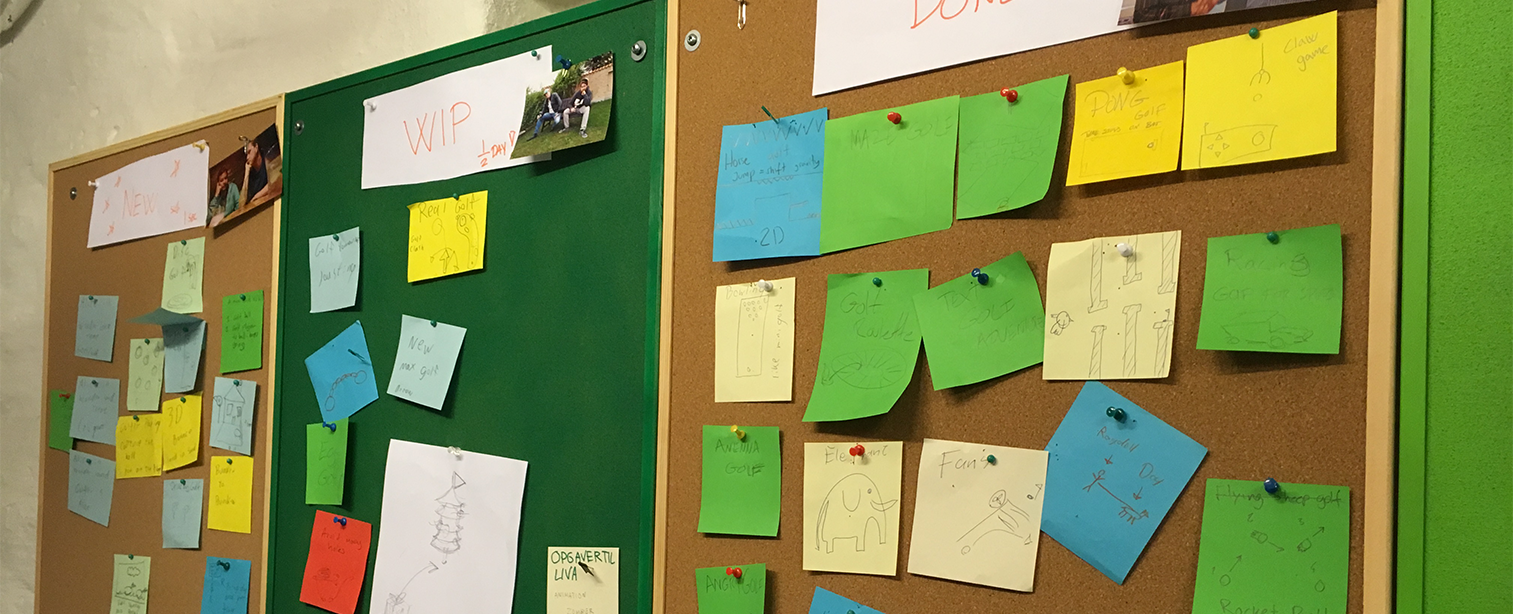
\includegraphics[width = \paperwidth]{Golf/Opslagstavle}}
    \caption{Bulletin Board for Golf Levels Ordered by New Ideas, Work in Progress and Done}
    \label{Bulletin}
  \end{figure}
\end{center}
\subsubsection{Paper Plane Golf}
My first idea for a level was one where the golf ball is a paper plane. You act on the plane by blowing wind behind it. The direction you shoot and the amount you pull back determines the wind direction and the blow force of the wind. The challenge is to go through some hoops as you make it to the flag at the end of the level. If you fall too far down the player gets reset and if the player blows in a direction too disparate from the direction the plane is heading, the blow force is lessened, simulating a similar situation in the real world.

Being the first level most of the challenges were getting an overview of how the pre-existing assets could aid me in the creation. As examples: The ground shape creation tool, the golf shooter and controller base class, The triggers used for triggering an out-of-bounds-event and the tags used for identifying elements such as golf balls and golf goals. As I have experienced in other projects, disarray has a way of sneaking into planned structures, and this was true also for this project but in a much more limited way than I had previously experienced. Even this small amount of disorder, however, spurred a tidying some time midway in my internship, further instilling a respect for order in me.

Another challenge that arose from the paper plane level, was the fact that a locked outlook behind a propelled object, does not allow for much relative perspective: As the paper plane approached the hoops I had positioned in the sky, it proved hard to judge the relative distance between the paper plane and the hoop, resulting in premature or late actions. Pitching the view forward solved this challenge slightly, but made planning ahead more difficult, since an approaching hoop was only apparent as the paper plane neared it. Since, however, any polish of levels was not part of the current development cycle, this status was deemed good enough, and I moved on to a new level.
\begin{center}
  \begin{figure}[!htb]
    \noindent\makebox[\textwidth]{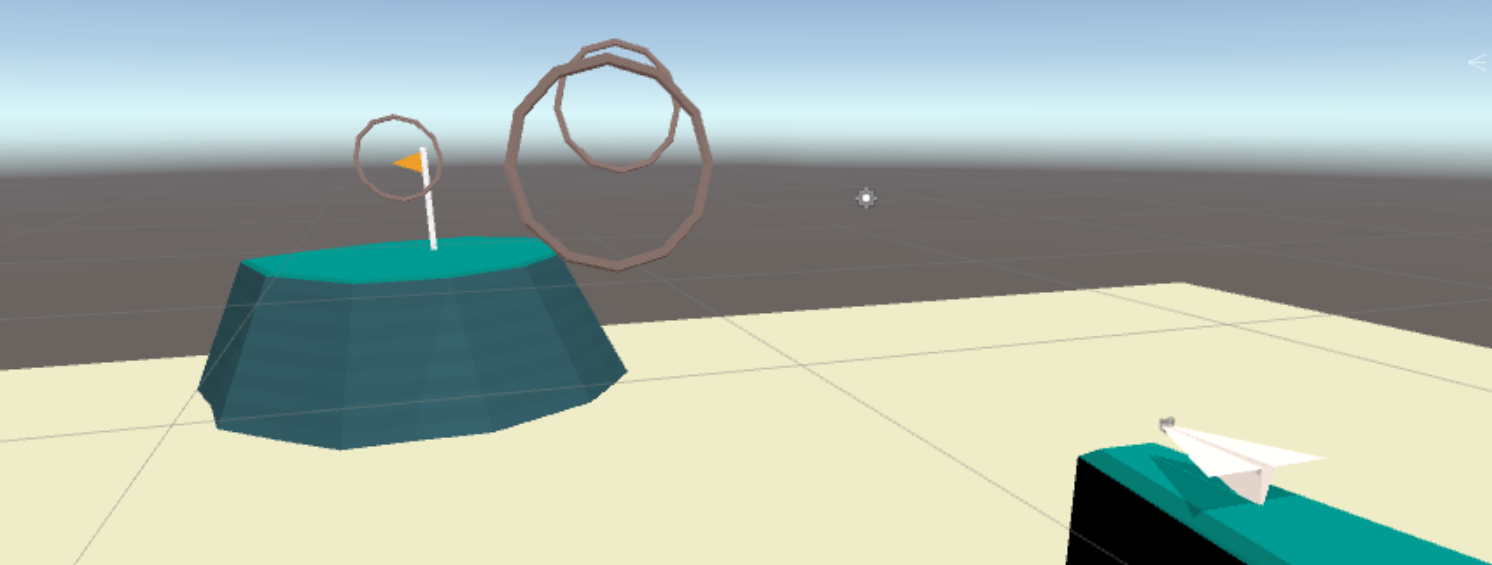
\includegraphics[width = \paperwidth]{Golf/PaperPlane}}
    \caption{The Paper Plane Level}
    \label{PaperPlane}
  \end{figure}
\end{center}
\subsubsection{Fishing Golf}
Next, was Fishing Golf. Here, the golf game was meant to be put in the context of a fishing trip. The first idea was a level in a first-person perspective and using the mobile device's gyroscope to look around. The goal was for the player to shoot out his/her fishing floater into the area where the water signalled the presence of fish. When the fish had latched on to the hook, the player should reel in the fish - level complete. This level proved to mainly be challenging in the creation of \textit{signifiers} \cite{norman}. Generally, there were three challenges in regards to signifiers: 1) Signalling the presence of fish in a certain area of the water. 2) Indicating that a fish had latched onto the hook. 3) Illustrating that having reeled in the fish completes the level. The first challenge was tackled by giving the visual cue of small waves, the second challenge I dealt with by using the vibration functionality of the mobile device, and the third challenge, the other intern and me tackled by modelling a fish that resembled the flag model from previous levels (see figure \ref{Fishing}). All in all, utilising a \textit{semantic} approach of using the player's connotations to the real world, with the waves that fish normally creates and the vibration simulating the pull on a fishing rod, and to the previous levels with the affinity of the fish to the flags \cite{semantics}.

After finishing the first-person level, we realised that there was more content in the fishing context. The next level the roles were switched and the player should now act as the fish in the water, but to complete the level the fish and the fisher should still meet. This time, however, the meeting place would be in the water. When the player manages to manoeuvre the fish into the hook, the force of the swimming fish will pull the fisher, now a golf ball, into the water and out of the safety of his boat (see figure \ref{Fishing}). Now, the player is able to connect the flag fish and the fisher golf ball and complete the level. This level, much like the last relies heavily on the player's ability of association, i.e. it is assumed that it should be intuitive at this point of the game progression, that a golf ball must meet a golf goal to complete the level.
\begin{center}
  \begin{figure}[!htb]
    \noindent\makebox[\textwidth]{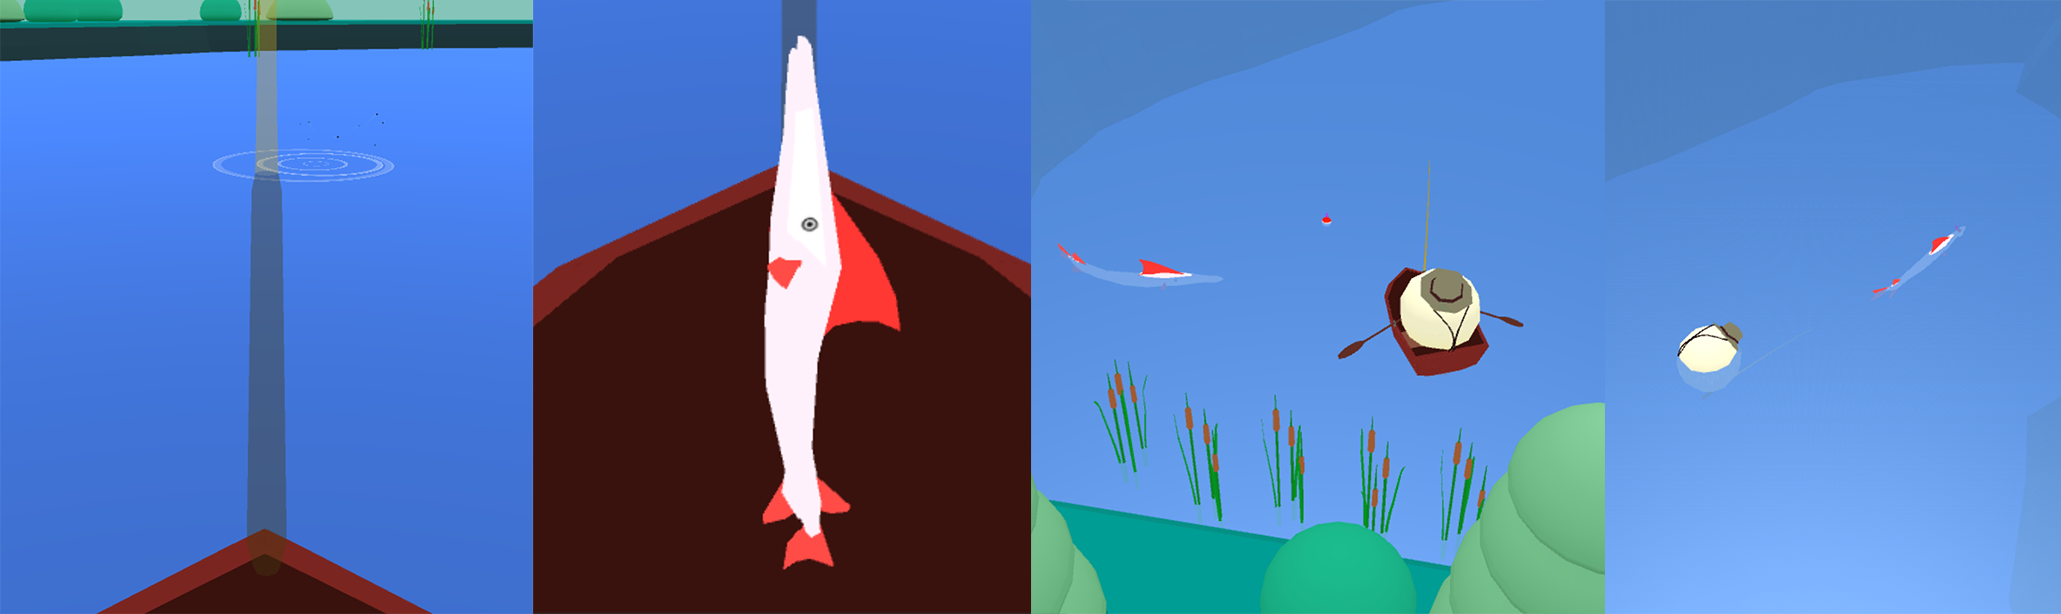
\includegraphics[width = \paperwidth]{Golf/Fishing}}
    \caption{Left: First-Person Fishing. Right: Golfing as a Fish}
    \label{Fishing}
  \end{figure}
\end{center}
\subsubsection{Domino Golf}
Domino is a game of its own, but the domino pieces themselves can also be used to create a sequence of aligned pieces that when toppled creates a satisfying domino effect, hence the name of the effect. For this level, I wanted to capture this feeling. I quickly realised, 1) that the game engine on its own could not quite capture this satisfactory collision when ivory meets ivory, and 2) the arduous work of aligning massive amounts of domino pieces. Thus, the first two challenges were identified. In addition to the first challenge, I also wanted to incorporate scale as an element in the collision feel: Small pieces colliding with other small pieces should progress fast and the opposite for large pieces, therefore I tied the overall timescale with the most current collision, so that, the smaller the piece the faster time progressed. This gave the desired illusion but proved ill-fitting when other elements undesirably got drawn into this time altering. Instead, a combination of increasing or decreasing the piece's velocity and the gravity acted upon it according to the piece's scale was implemented. For the second challenge I needed a tool that could assist in setting up the domino pieces in a line, but not a straight line. I implemented a method that could place domino pieces according to an unlimited amount of segments containing a Bezier curve. Further, I made the line visible in a simplified version outside of play mode, to better determine the path. Finally, I made an accompanying two-dimensional graph for determining scale in the course of the line.

Next, was the problem of what to control. I determined that it should be a domino piece, and this proved to be difficult because of the shape. It is quite difficult to build up speed when the dimensions of the projectile are highly unbalanced. The long rectangular shape of a domino piece, simply, is not made for speed. This meant that the first iteration of the domino controller felt very much like a fish out of water, not meant to travel across the ground. At this point, I was trying to determine whether or not this was what I wanted. After all, a golf field is not a domino piece's natural habitat. I decided to iterate nonetheless: Instead of just forcing the piece across the level, I decided to, when the player touches the screen, alter the posture of the piece to a standing one, and then when the player releases, boost the piece forward in a handspring-manner (flick flack). This felt extremely satisfying and how I felt a domino piece would traverse a golf field.
\begin{center}
  \begin{figure}[!htb]
    \noindent\makebox[\textwidth]{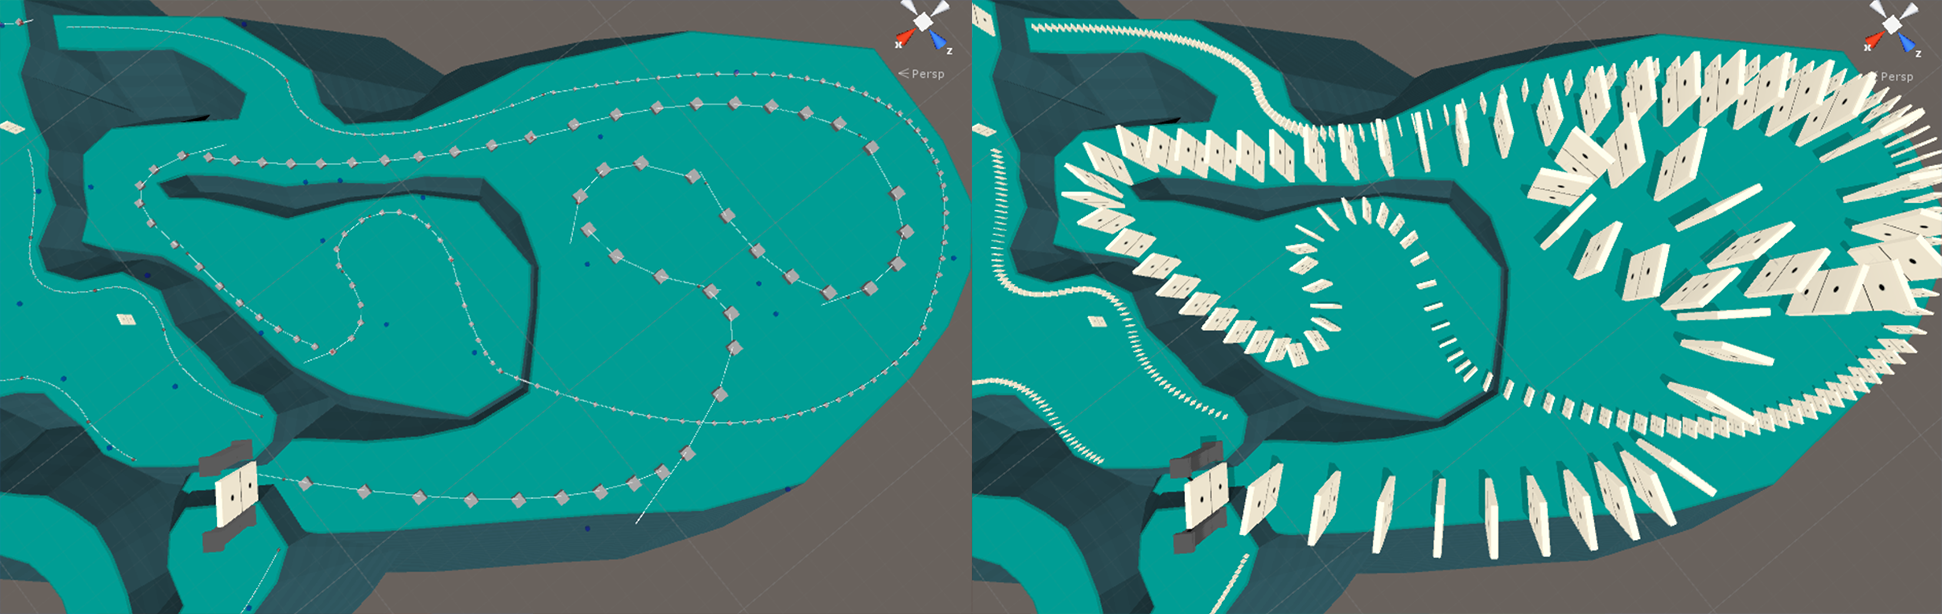
\includegraphics[width = \paperwidth]{Golf/Domino}}
    \caption{Left: Domino Pieces Visualised outside of Play Mode. Right: In Play Mode}
    \label{Domino}
  \end{figure}
\end{center}
\subsubsection{Dash Golf}
After having spent time working on a pleasing shooting mechanic for a domino piece, I wanted to do the same thing for the regular golf ball. Having noticed a growing concerned in the office, about very few levels taking advantage of not necessarily shooting at full velocity, i.e. most levels had a dominant strategy of always shooting at maximum speed, I wanted to make a level where this was not true. Another thing I noticed was the scarcity of levels taking advantage of verticality. These observations lead to a shooting mechanic with two features: 1) When the player touches a point on the screen, the ball lifts a meter off the ground and starts levitating here. Then, depending on how far the player pulls and releases, the ball dashes a certain distance through the air, halts and floats back to the ground. 2) Should the ball hit a green wall with a number on it, the number decreases by one, and the ball slams into the wall and recoils back and up. Should the player then touch the screen just after the impact the ball flies one meter up again, but this time from the point of impact, giving it another meter of verticality. It is then possible to climb these walls until the number reaches zero (see figure \ref{Dash}).

To convey this mechanic to the player, I chose the colour green to be the carrier of meaning in all aspects. When the ball is lying dormant and when it levitates in the air there is a green glow emanating from the ball, signifying that this is not a regular golf ball. When the ball has been shot, the green glow disappears and only reappears if the ball touches the ground or a green wall, signifying that its ability to dash relies on the contact of one of these. The walls are also green to signify the connection between the dash ability and the wall.
\begin{center}
  \begin{figure}[!htb]
    \noindent\makebox[\textwidth]{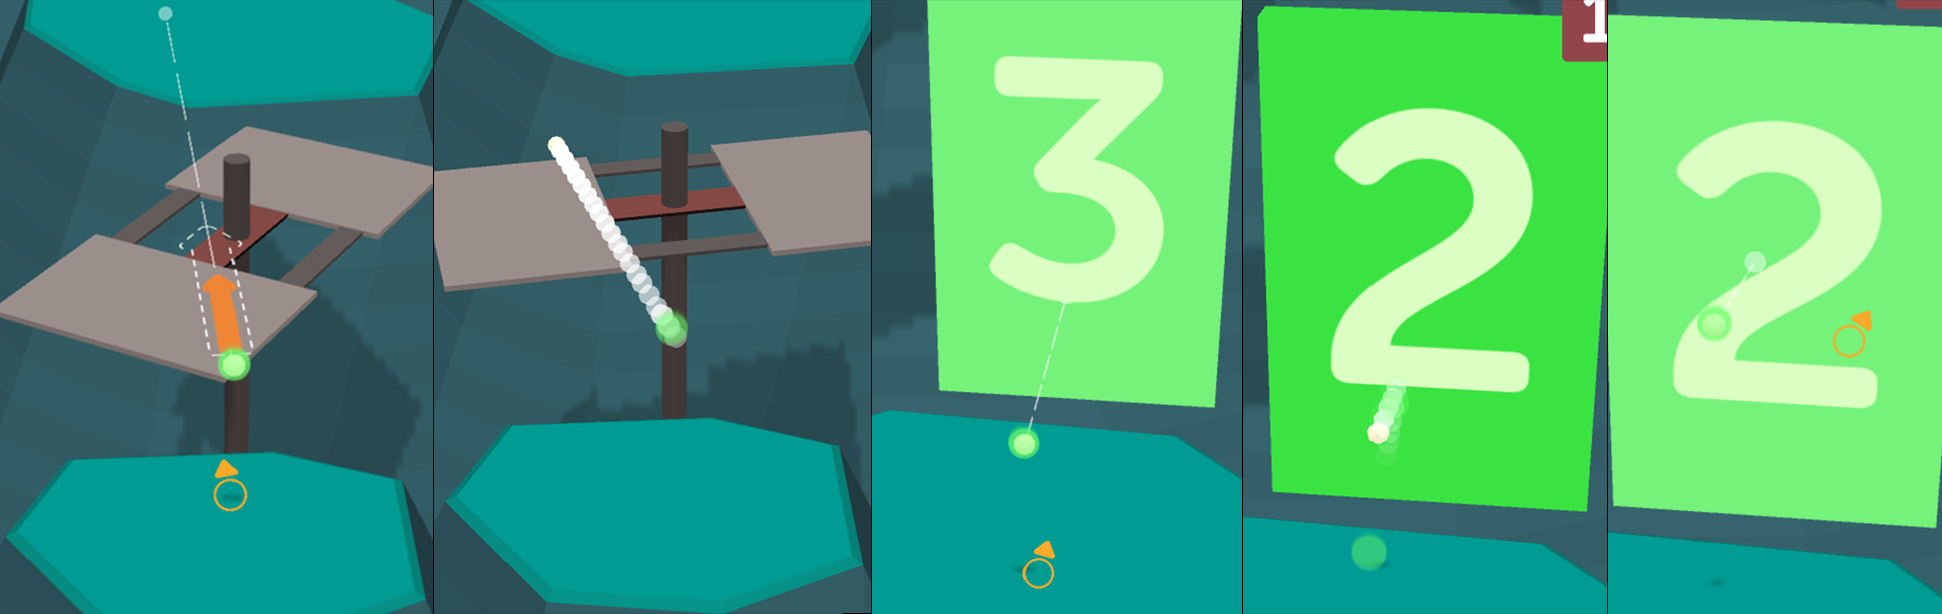
\includegraphics[width = \paperwidth]{Golf/Dash}}
    \caption{Left: The Dash Shoot and Aim Mechanic. Right: Hitting a Green Wall}
    \label{Dash}
  \end{figure}
\end{center}
